\chapter{DỮ LIỆU VÀ PHƯƠNG PHÁP}
\label{ch:phuong_phap}

\section{Bộ dữ liệu}

\subsection{Nguồn và quy mô}

Đề tài sử dụng bộ dữ liệu \textit{pkdarabi/cardetection} công bố trên Kaggle, phân phối dưới dạng
một bản xuất Roboflow theo bố cục thư mục chuẩn \texttt{\{train,valid,test\}/\{images,labels\}} với
nhãn ở định dạng YOLO TXT. Mặc dù tên trên đường dẫn là ``car detection'', nội dung thực tế của
toàn bộ 15 lớp đều là đèn tín hiệu và biển giới hạn tốc độ, không có lớp nào là phương tiện. Nhóm
thực hiện giữ nguyên 15 lớp gốc, không gộp cũng không ánh xạ lại nhãn, để kết quả có thể đối chiếu
với các công bố khác dùng cùng bộ dữ liệu.

\begin{table}[H]
\centering
\caption{Thống kê tổng quan bộ dữ liệu theo từng tập}
\label{tab:dataset_summary}
\small
\begin{tabular}{lrrrr}
\toprule
\textbf{Tập} & \textbf{Số ảnh} & \textbf{Tỉ lệ} & \textbf{Số hộp bao} & \textbf{Hộp/ảnh} \\
\midrule
Huấn luyện & 3.530 & 71,0\% & 4.298 & 1,218 \\
Kiểm định  & 801   & 16,1\% & 944   & 1,179 \\
Kiểm tra   & 638   & 12,8\% & 770   & 1,207 \\
\midrule
\textbf{Tổng} & \textbf{4.969} & \textbf{100\%} & \textbf{6.012} & \textbf{1,210} \\
\bottomrule
\end{tabular}
\end{table}

Toàn bộ ảnh có độ phân giải đồng nhất 416$\times$416 điểm ảnh --- hệ quả của bước tiền xử lý mà
Roboflow áp dụng khi xuất bộ dữ liệu. Chi tiết này có một hệ quả kỹ thuật đáng lưu ý: việc tăng
kích thước ảnh đầu vào khi huấn luyện chủ yếu là phóng to chứ không bổ sung thêm chi tiết thật.

Mật độ vật thể rất thưa: trung bình chỉ 1,21 hộp bao trên mỗi ảnh, cao nhất là 10 hộp ở tập kiểm
tra. Đây là đặc điểm khác hẳn các bộ dữ liệu cảnh đường phố như TT100K~\cite{zhu2016tt100k}, nơi
một khung hình có thể chứa hàng chục biển báo.

\subsection{Phân bố lớp và mất cân bằng}

\begin{figure}[H]
\centering
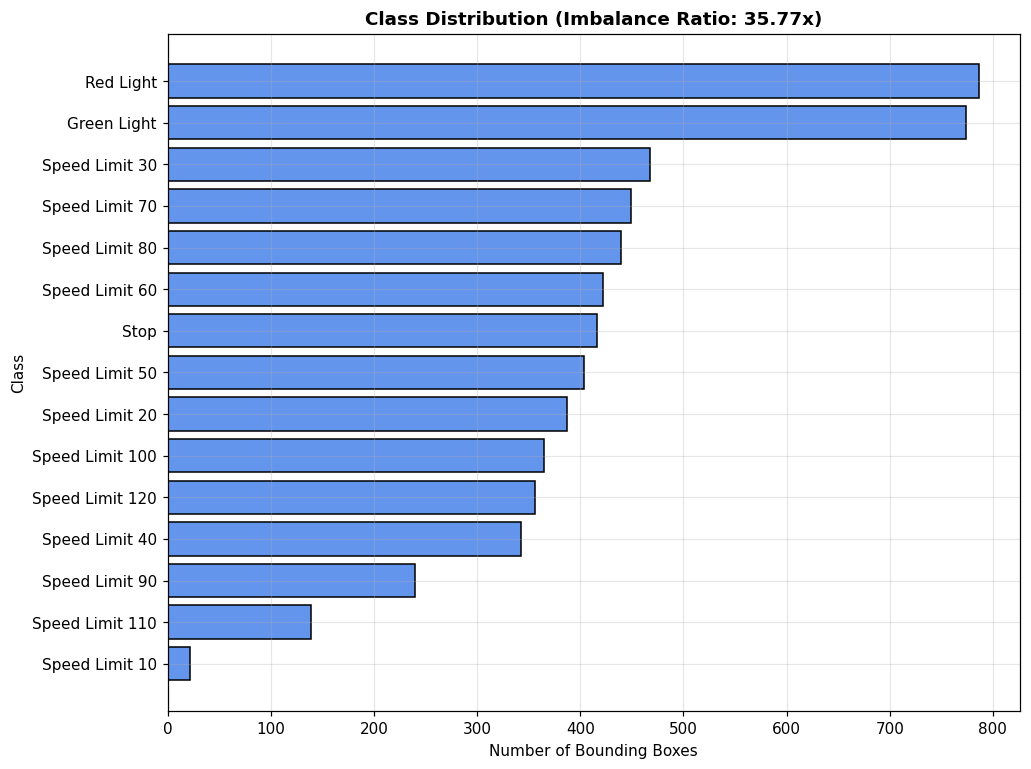
\includegraphics[width=0.92\textwidth]{figures/eda_class_distribution.png}
\caption{Phân bố số hộp bao theo từng lớp trên toàn bộ dữ liệu}
\label{fig:class_dist}
\end{figure}

Hình~\ref{fig:class_dist} và Bảng~\ref{tab:class_dist} cho thấy mức mất cân bằng đáng kể. Hai lớp
đèn tín hiệu chiếm gần 26\% tổng số hộp bao, trong khi lớp \textit{Speed Limit 10} chỉ có 22 mẫu,
tương đương 0,37\%. Tỉ số mất cân bằng, định nghĩa bằng thương giữa số mẫu của lớp nhiều nhất và
lớp ít nhất, đạt \textbf{35,77}.

\begin{table}[H]
\centering
\caption{Phân bố lớp chi tiết, sắp theo số hộp bao giảm dần}
\label{tab:class_dist}
\small
\begin{tabular}{clrrr}
\toprule
\textbf{Mã lớp} & \textbf{Tên lớp} & \textbf{Số hộp} & \textbf{Tỉ lệ (\%)} & \textbf{Tỉ số so với lớp lớn nhất} \\
\midrule
1  & Red Light        & 787 & 13,09 & 1,00 \\
0  & Green Light      & 774 & 12,87 & 1,02 \\
7  & Speed Limit 30   & 468 & 7,78  & 1,68 \\
11 & Speed Limit 70   & 449 & 7,47  & 1,75 \\
12 & Speed Limit 80   & 440 & 7,32  & 1,79 \\
10 & Speed Limit 60   & 422 & 7,02  & 1,86 \\
14 & Stop             & 416 & 6,92  & 1,89 \\
9  & Speed Limit 50   & 404 & 6,72  & 1,95 \\
6  & Speed Limit 20   & 387 & 6,44  & 2,03 \\
3  & Speed Limit 100  & 365 & 6,07  & 2,16 \\
5  & Speed Limit 120  & 356 & 5,92  & 2,21 \\
8  & Speed Limit 40   & 343 & 5,71  & 2,29 \\
13 & Speed Limit 90   & 240 & 3,99  & 3,28 \\
4  & Speed Limit 110  & 139 & 2,31  & 5,66 \\
2  & Speed Limit 10   & 22  & 0,37  & \textbf{35,77} \\
\bottomrule
\end{tabular}
\end{table}

Khi cài đặt phép tính này, một chi tiết dễ sai đã được xử lý tường minh: nếu chỉ đếm các lớp thực sự
xuất hiện trong dữ liệu, một lớp được khai báo trong tệp cấu hình nhưng không có mẫu nào sẽ bị âm
thầm bỏ qua, khiến tỉ số mất cân bằng bị báo cáo thấp hơn thực tế và ``lớp hiếm nhất'' bị xác định
sai. Mô-đun phân tích do đó đánh chỉ mục lại bảng đếm theo toàn bộ tập lớp khai báo với giá trị mặc
định bằng không, và trả về vô cùng khi có lớp rỗng.

\subsection{Thống kê kích thước hộp bao}

\begin{figure}[H]
\centering
\begin{subfigure}[b]{0.48\textwidth}
  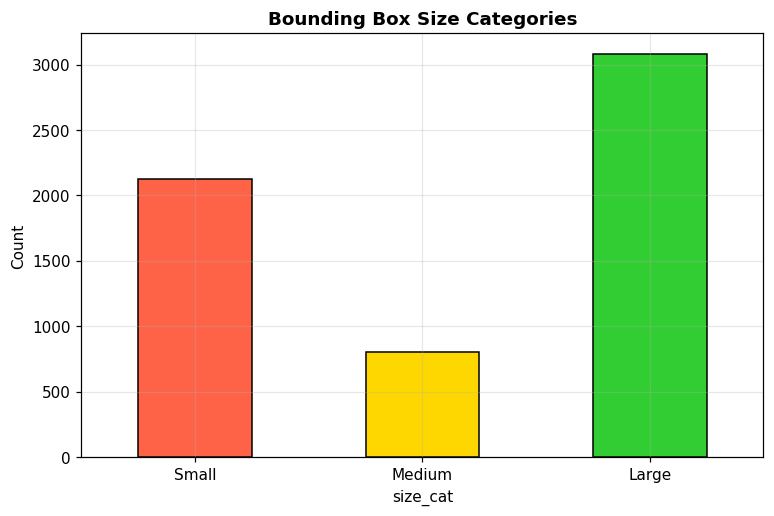
\includegraphics[width=\textwidth]{figures/eda_bbox_size_categories.png}
  \caption{Phân nhóm kích thước}
\end{subfigure}
\hfill
\begin{subfigure}[b]{0.48\textwidth}
  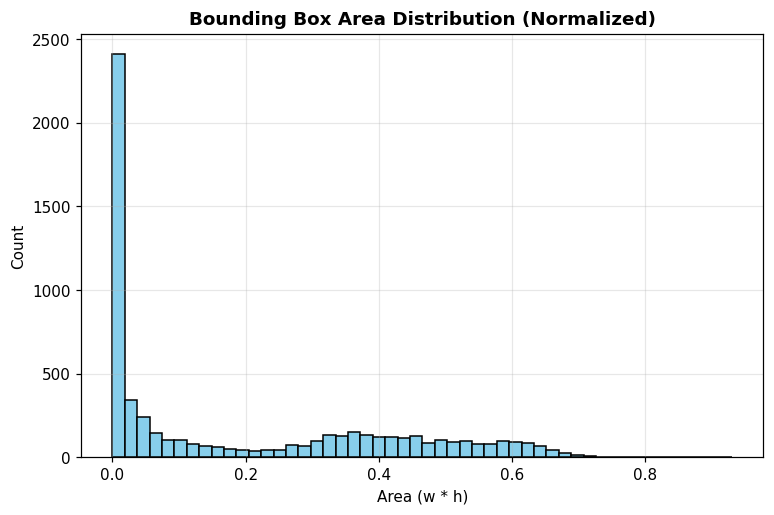
\includegraphics[width=\textwidth]{figures/eda_bbox_area.png}
  \caption{Phân bố diện tích chuẩn hoá}
\end{subfigure}
\caption{Thống kê kích thước hộp bao trên toàn bộ dữ liệu}
\label{fig:bbox_size}
\end{figure}

Việc phân nhóm kích thước ở bước khám phá dữ liệu dùng diện tích đã chuẩn hoá $a = w \cdot h$ với
$w, h \in [0,1]$, theo ba ngưỡng: nhỏ khi $a < 0{,}01$, trung bình khi $0{,}01 \le a < 0{,}05$, và
lớn trong các trường hợp còn lại. Cần lưu ý rằng quy ước này khác với quy ước COCO ở
biểu thức~\eqref{eq:apsize}, vốn dùng diện tích tuyệt đối theo điểm ảnh. Lựa chọn dùng diện tích
chuẩn hoá ở đây là có chủ ý: nó độc lập với độ phân giải ảnh nên so sánh được giữa các nguồn dữ
liệu khác nhau. Khi tính $AP$ ở Chương~\ref{ch:ket_qua} thì quy ước COCO được dùng.

\begin{table}[H]
\centering
\caption{Phân nhóm kích thước hộp bao theo diện tích chuẩn hoá}
\label{tab:bbox_cat}
\small
\begin{tabular}{lrrl}
\toprule
\textbf{Nhóm} & \textbf{Số hộp} & \textbf{Tỉ lệ (\%)} & \textbf{Ngưỡng diện tích chuẩn hoá} \\
\midrule
Nhỏ        & 2.122 & 35,30 & $a < 0{,}01$ \\
Trung bình & 806   & 13,41 & $0{,}01 \le a < 0{,}05$ \\
Lớn        & 3.084 & 51,30 & $a \ge 0{,}05$ \\
\bottomrule
\end{tabular}
\end{table}

Bảng~\ref{tab:bbox_cat} chứa một tín hiệu bất thường. Trong một bộ dữ liệu cảnh đường phố thông
thường, nhóm vật thể lớn hiếm khi chiếm quá bán, bởi biển báo chiếm hơn 5\% diện tích khung hình
đồng nghĩa với việc xe đã ở rất gần biển. Ở đây nhóm lớn chiếm tới 51,30\%. Điều này thúc đẩy phân
tích ở mục tiếp theo.

\subsection{Phân tích thành phần bộ dữ liệu}
\label{sec:thanhphan}

Quan sát tên tệp cho thấy bộ dữ liệu không đồng nhất mà là một tập \emph{trộn} từ nhiều nguồn có
quy ước đặt tên khác nhau. Nhóm thực hiện phân loại ảnh theo mẫu tên tệp và tính lại thống kê kích
thước riêng cho từng nhóm; kết quả trình bày ở Bảng~\ref{tab:thanhphan}.

\begin{table}[H]
\centering
\caption{Thành phần bộ dữ liệu theo nguồn gốc suy ra từ quy ước đặt tên tệp}
\label{tab:thanhphan}
\small
\begin{tabular}{lrrrr}
\toprule
\textbf{Nhóm nguồn} & \textbf{Số ảnh} & \textbf{Tỉ lệ (\%)} & \textbf{Cạnh biển (trung vị)} & \textbf{\% vật thể nhỏ} \\
\midrule
Ảnh cắt kiểu GTSRB & 1.922 & 38,68 & 66,8\% cạnh ảnh & 0,0 \\
Ảnh số sáu chữ số  & 1.586 & 31,92 & 19,6\%          & 34,7 \\
Ảnh cảnh đường     & 724   & 14,57 & 13,4\%          & 31,1 \\
Camera mắt cá      & 645   & 12,98 & 1,6\%           & 99,6 \\
Nhóm khác          & 92    & 1,85  & 75,7\%          & 0,0 \\
\bottomrule
\end{tabular}
\end{table}

Kết quả này giải thích trọn vẹn hình dạng bất thường ở Bảng~\ref{tab:bbox_cat}. Nhóm ảnh cắt kiểu
GTSRB chiếm 38,68\% số ảnh và có biển báo lấp gần kín khung hình --- đây vốn là ảnh dành cho bài
toán \emph{phân lớp} chứ không phải \emph{phát hiện}~\cite{stallkamp2012gtsrb}. Ở đầu kia của thang
đo, nhóm camera mắt cá có tới 99,6\% vật thể thuộc nhóm nhỏ, với cạnh biển trung vị chỉ 1,6\% cạnh
ảnh, đồng thời mang hình học quang học hoàn toàn khác.

Hệ quả là phân bố kích thước bị \emph{lưỡng cực}. Bảng~\ref{tab:percentile} trình bày các phân vị
diện tích quy đổi ra cạnh tính bằng điểm ảnh trên ảnh 416$\times$416.

\begin{table}[H]
\centering
\caption{Phân vị diện tích hộp bao và cạnh tương ứng trên ảnh 416$\times$416}
\label{tab:percentile}
\small
\begin{tabular}{lrrrrr}
\toprule
\textbf{Phân vị} & \textbf{10\%} & \textbf{25\%} & \textbf{50\%} & \textbf{75\%} & \textbf{90\%} \\
\midrule
Diện tích chuẩn hoá & 0,0003 & 0,0025 & 0,0570 & 0,3854 & 0,5402 \\
Cạnh tương ứng (điểm ảnh) & 6,9 & 20,8 & 99,3 & 258,2 & 305,8 \\
\bottomrule
\end{tabular}
\end{table}

Khoảng cách giữa phân vị 25\% (20,8 điểm ảnh) và phân vị 75\% (258,2 điểm ảnh) là hơn mười hai lần,
và vùng ``biển báo thật trên đường'' --- khoảng 30 đến 80 điểm ảnh --- gần như trống. Đây là một
dạng thiên lệch bộ dữ liệu điển hình~\cite{torralba2011bias}, và nó có hai hệ quả đối với đề tài
này. Thứ nhất, hơn một nửa vật thể thuộc nhóm lớn nên mAP tổng bị chi phối bởi các trường hợp dễ.
Thứ hai, chính vì vậy mà việc tách $AP$ theo nhóm kích thước như đã lập luận ở
Mục~\ref{sec:ap_theo_kichthuoc} trở thành bắt buộc chứ không phải tuỳ chọn.

\begin{figure}[H]
\centering
\begin{subfigure}[b]{0.32\textwidth}
  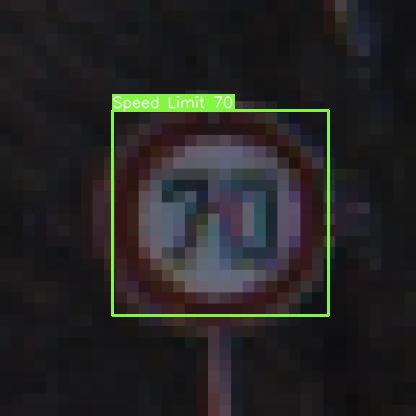
\includegraphics[width=\textwidth]{figures/sample_gtsrb_crop.jpg}
  \caption{Ảnh cắt kiểu GTSRB}
\end{subfigure}
\hfill
\begin{subfigure}[b]{0.32\textwidth}
  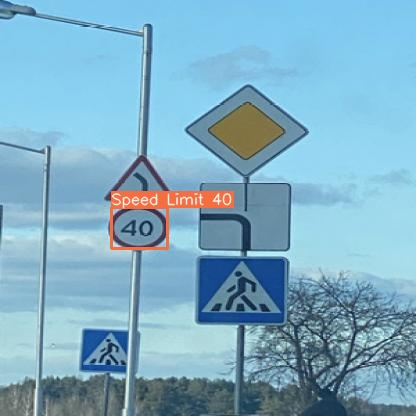
\includegraphics[width=\textwidth]{figures/sample_road_scene.jpg}
  \caption{Ảnh cảnh đường}
\end{subfigure}
\hfill
\begin{subfigure}[b]{0.32\textwidth}
  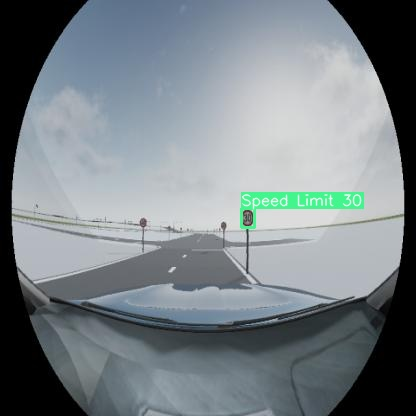
\includegraphics[width=\textwidth]{figures/sample_fisheye.jpg}
  \caption{Camera mắt cá}
\end{subfigure}
\caption{Ba chế độ ảnh cùng tồn tại trong bộ dữ liệu, kèm hộp bao nhãn thật}
\label{fig:ba_che_do}
\end{figure}

\subsection{Vị trí vật thể trong khung hình}

\begin{figure}[H]
\centering
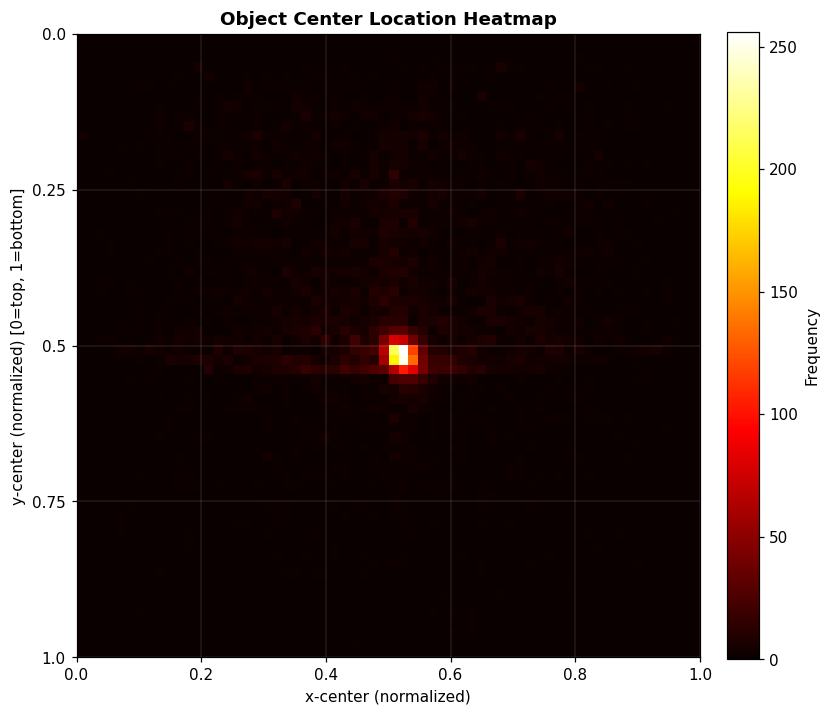
\includegraphics[width=0.62\textwidth]{figures/eda_object_center_heatmap.png}
\caption{Bản đồ nhiệt vị trí tâm vật thể trên toàn bộ dữ liệu}
\label{fig:heatmap}
\end{figure}

Bản đồ nhiệt ở Hình~\ref{fig:heatmap} được xây bằng biểu đồ tần suất hai chiều trên toạ độ tâm đã
chuẩn hoá. Hai chi tiết cài đặt cần lưu ý. Thứ nhất, trục tung được lật theo phép $y' = 1 - y_c$ vì
hệ toạ độ ảnh đặt gốc ở góc trên trái với trục $y$ hướng xuống, trong khi hệ toạ độ đồ thị hướng
lên. Thứ hai, ma trận tần suất phải được chuyển vị trước khi hiển thị, do hàm dựng biểu đồ hai
chiều trả về theo thứ tự (trục hoành, trục tung) còn hàm hiển thị ảnh yêu cầu thứ tự (hàng, cột).
Bỏ qua một trong hai bước này sẽ cho một bản đồ nhiệt trông hợp lý nhưng sai hoàn toàn về mặt hình
học.

Điểm nóng tập trung mạnh ở vùng trung tâm, phản ánh đúng thành phần dữ liệu đã phân tích ở
Mục~\ref{sec:thanhphan}: nhóm ảnh cắt kiểu GTSRB luôn đặt biển báo ở giữa khung hình.

\subsection{Kiểm tra chất lượng nhãn}

Một mô-đun kiểm tra độc lập rà soát tám loại lỗi: thiếu ảnh, thiếu nhãn, nhãn rỗng, ảnh hỏng, trùng
tên ảnh giữa các tập, mã lớp ngoài miền hợp lệ, toạ độ hộp nằm ngoài đoạn $[0,1]$ và hộp có cạnh
bằng không.

Kết quả trên cả ba tập đều sạch về mặt hình học: không có hộp suy biến, không có mã lớp sai. Chỉ
ghi nhận \textbf{4 ảnh có tệp nhãn rỗng}, tức ảnh nền không chứa biển báo nào --- đây không phải lỗi
mà là ảnh nền hợp lệ, thường được giữ lại có chủ đích để giảm dương tính giả.

Về mặt cài đặt, việc đối chiếu tên ảnh với tên tệp nhãn dùng cấu trúc tập hợp thay vì danh sách,
nhờ đó phép kiểm tra thành viên có độ phức tạp hằng số thay vì tuyến tính, tránh chi phí bậc hai
khi quy mô dữ liệu tăng.

\subsection{Kiểm toán rò rỉ dữ liệu giữa các tập}
\label{sec:kiem_toan_ro_ri}

Một thủ tục kiểm toán riêng được thực hiện để phát hiện ảnh xuất hiện ở nhiều hơn một tập --- vấn đề
đã được ghi nhận là nguồn thổi phồng chỉ số trên nhiều bộ chuẩn phổ biến~\cite{barz2020duplicates}.
Thủ tục đối chiếu theo hai mức: tên ảnh nguồn sau khi loại bỏ hậu tố ngẫu nhiên do Roboflow thêm
vào, và băm nội dung tệp để xác định các cặp trùng byte hoàn toàn. Kết quả được trình bày ở
Mục~\ref{sec:trai_ky_vong} và ảnh hưởng trực tiếp tới cách diễn giải mọi chỉ số trong báo cáo.

\section{Thiết kế thực nghiệm}

\subsection{Năm cấu hình khảo sát}

Toàn bộ thực nghiệm được tổ chức thành một lượt chạy duy nhất sinh ra năm cấu hình, trình bày ở
Bảng~\ref{tab:cauhinh}. Việc gộp chung một lượt là có chủ đích: nó bảo đảm mọi cấu hình dùng cùng
một tập kiểm tra, cùng một phần cứng và cùng một bộ tính độ đo, nên chênh lệch quan sát được không
lẫn yếu tố môi trường.

\begin{table}[H]
\centering
\caption{Năm cấu hình khảo sát và vai trò của từng cấu hình}
\label{tab:cauhinh}
\small
\begin{tabular}{p{3.6cm} p{3.1cm} p{6.6cm}}
\toprule
\textbf{Cấu hình} & \textbf{Vai trò} & \textbf{Mục đích} \\
\midrule
YOLO26s            & Thầy            & Cung cấp phân phối mềm cho chưng cất; đồng thời là cận trên tham chiếu \\
YOLO26n            & Trò đối chứng   & Huấn luyện thông thường --- mốc so sánh cho giả thuyết chưng cất \\
YOLO26n + chưng cất& Trò chưng cất   & Cấu hình cần đánh giá của giả thuyết thứ nhất \\
ONNX FP32          & Xuất từ trò chưng cất & Tách riêng ảnh hưởng của việc đổi môi trường thực thi \\
ONNX INT8          & Xuất từ trò chưng cất & Cấu hình cần đánh giá của giả thuyết thứ hai \\
\bottomrule
\end{tabular}
\end{table}

Cần chú ý vai trò của cấu hình ONNX FP32: nó tồn tại để \emph{cô lập biến số}. Nếu chỉ so ONNX INT8
với mô hình PyTorch gốc, phần chênh lệch sẽ trộn lẫn hai nguyên nhân --- đổi môi trường thực thi và
lượng tử hoá. Có thêm mốc ONNX FP32 ở giữa cho phép quy phần chênh lệch giữa hai bản ONNX về đúng
tác động của lượng tử hoá.

\subsection{Siêu tham số}

\begin{table}[H]
\centering
\caption{Siêu tham số huấn luyện và đánh giá}
\label{tab:e3_cfg}
\small
\begin{tabular}{lll}
\toprule
\textbf{Tham số} & \textbf{Giá trị} & \textbf{Ghi chú} \\
\midrule
Mô hình thầy       & \texttt{yolo26s.pt} & 9,47 triệu tham số \\
Mô hình trò        & \texttt{yolo26n.pt} & 2,38 triệu tham số \\
Số chu kỳ          & 50 / 50 / 50 & Thầy, trò đối chứng, trò chưng cất --- bằng nhau \\
Kích thước lô      & 16 / 24 / \textbf{8} & \textbf{Không bằng nhau --- xem ghi chú bên dưới} \\
Kiên nhẫn dừng sớm & 12 & \\
Hệ số chưng cất    & 6,0 & Giá trị mặc định của thư viện \\
Kích thước ảnh     & 640 & \\
Hạt ngẫu nhiên     & 42 & Dùng chung cho toàn bộ đề tài \\
Ngưỡng tin cậy khi đo & 0,001 & Gần bằng không, phù hợp với độ đo xếp hạng \\
Ngưỡng IoU khi khớp   & 0,50 & \\
Số ảnh hiệu chuẩn INT8 & 300 & \\
Số lượt khởi động / đo tốc độ & 10 / 100 & \\
\bottomrule
\end{tabular}
\end{table}

Cả ba nhánh huấn luyện đều dùng bộ tăng cường dữ liệu mặc định của thư viện, trong đó có phép ghép
ảnh mosaic phổ biến từ YOLOv4~\cite{bochkovskiy2020yolov4} --- kỹ thuật ghép bốn ảnh thành một, vừa
tăng số ngữ cảnh nền mà mỗi vật thể xuất hiện, vừa tạo ra các vật thể ở tỉ lệ nhỏ hơn. Việc giữ
nguyên cùng một bộ tăng cường cho cả ba nhánh là điều kiện cần để so sánh công bằng; nói chung,
tăng cường dữ liệu phải phù hợp với ngữ nghĩa của miền ứng dụng chứ không thể áp dụng máy
móc~\cite{shorten2019augmentation}.

Mô hình trò được huấn luyện \emph{hai lần} với cùng số chu kỳ, cùng hạt ngẫu nhiên và cùng kích
thước ảnh --- một lần thông thường và một lần bật chưng cất. Đây là điều kiện cần để chênh lệch
quan sát được quy về đúng biến số cần khảo sát.

Tuy nhiên cần nêu rõ một \textbf{yếu tố gây nhiễu chưa kiểm soát được}: nhánh chưng cất chạy với
kích thước lô bằng 8, trong khi nhánh đối chứng dùng 24. Nguyên nhân là trong quá trình chưng cất
phải nạp đồng thời cả mô hình thầy lẫn mô hình trò vào bộ nhớ card đồ hoạ. Vì kích thước lô ảnh
hưởng tới chất lượng ước lượng gradient, phần chênh lệch quan sát được ở Chương~\ref{ch:ket_qua}
không thể quy hoàn toàn cho bản thân kỹ thuật chưng cất. Đây là hạn chế được ghi nhận thay vì bỏ
qua.

\subsection{Ngưỡng chấp nhận khai báo trước}
\label{sec:nguong_chap_nhan}

Năm ngưỡng chấp nhận được khai báo \emph{trước} khi chạy thực nghiệm, ngay trong ô cấu hình đầu
tiên của sổ tay:

\begin{itemize}[leftmargin=1.5cm]
\item Mô hình chưng cất không được kém mô hình đối chứng quá 0,005 điểm mAP@0,5:0,95.
\item Mô hình chưng cất được kỳ vọng \emph{tốt hơn} mô hình đối chứng.
\item Bản INT8 không được giảm quá 0,015 điểm mAP so với bản FP32.
\item Bản INT8 phải nhỏ hơn bản FP32 ít nhất 50\% về dung lượng tệp.
\item Mô hình trò phải nhẹ hơn mô hình thầy.
\end{itemize}

Cách làm này buộc người thực hiện cam kết tiêu chí đánh giá trước khi nhìn thấy số liệu, tránh việc
điều chỉnh kỳ vọng cho khớp với kết quả thu được. Kết quả kiểm tra được báo cáo đầy đủ ở
Chương~\ref{ch:ket_qua}, kể cả các ngưỡng không đạt.

\subsection{Quy trình đánh giá}

Toàn bộ năm cấu hình được đánh giá trên tập kiểm tra tách biệt bằng \textbf{pycocotools}, sau khi
nhãn YOLO được chuyển sang định dạng COCO theo biểu thức~\eqref{eq:yolo2coco}. Lựa chọn này quan
trọng vì hai lý do. Thứ nhất, nó cho $AP$ tách theo ba nhóm kích thước theo quy ước ở
biểu thức~\eqref{eq:apsize} --- chỉ số trung tâm của đề tài. Thứ hai, dùng một bộ đánh giá duy nhất
cho cả mô hình PyTorch lẫn mô hình ONNX loại bỏ khả năng chênh lệch đến từ hai cài đặt mAP khác
nhau.

Ngưỡng tin cậy khi đo được đặt bằng 0,001, tức gần như không lọc. Đây là điểm dễ gây hiểu nhầm nên
cần nói rõ: mAP là độ đo xếp hạng, cần trọn bộ dự đoán có điểm số để dựng đầy đủ đường cong PR. Lọc
theo ngưỡng tin cậy trước khi tính sẽ cắt mất phần đuôi độ bao phủ và làm sai lệch chỉ số. Ngưỡng
tin cậy cao hơn chỉ được dùng ở khâu trình diễn trực quan.

Tốc độ suy luận được đo bằng cách chạy 100 lượt truyền xuôi sau 10 lượt khởi động, rồi lấy trung vị
và phân vị 95\%. Giai đoạn khởi động là bắt buộc vì lượt chạy đầu tiên chịu chi phí khởi tạo ngữ
cảnh tính toán và dò thuật toán, sẽ làm phồng số đo nếu không loại bỏ.

\subsection{Bảo đảm tính tái lập}

Ba biện pháp được áp dụng. Thứ nhất, một hàm gieo hạt duy nhất đặt hạt cho biến môi trường băm của
Python, thư viện ngẫu nhiên chuẩn, NumPy, PyTorch~\cite{paszke2019pytorch} và PyTorch CUDA, đồng
thời bật chế độ tất định của cuDNN và \emph{tắt} chế độ tự dò thuật toán nhanh nhất. Việc tắt chế
độ tự dò là cần thiết vì nó chọn thuật toán tích chập theo điều kiện thực thi tại thời điểm chạy,
khiến kết quả không lặp lại được giữa các lần. Hạt mặc định là 42.

Thứ hai, mọi đường dẫn đầu vào và đầu ra được khai báo tại một nơi duy nhất, có hỗ trợ biến môi
trường để cùng một mã nguồn chạy được trên nhiều nền tảng.

Ngoài ra, bộ tối ưu và lịch tốc độ học được giữ ở cấu hình mặc định của thư viện cho cả ba nhánh;
họ thuật toán Adam có tách rời suy giảm trọng số~\cite{loshchilov2019adamw} là lựa chọn tiêu chuẩn
trong bối cảnh này.

Thứ ba, quy trình được chia thành các giai đoạn có đánh dấu hoàn thành, cho phép chạy lại từng phần
mà không phải huấn luyện lại từ đầu --- hữu ích khi phiên làm việc bị ngắt giữa chừng.
